\documentclass[conference]{IEEEtran}
\usepackage[utf8]{inputenc}
\usepackage[T1]{fontenc}
\usepackage{amsmath,amssymb}
\usepackage{graphicx}
\usepackage{booktabs}
\usepackage{multirow}
\usepackage{cite}
\usepackage{xcolor}
\usepackage[hidelinks]{hyperref}
\newcommand{\pend}[1]{\textcolor{red}{[#1]}}
\newcommand{\pmsd}[2]{$#1 \pm #2$}

\begin{document}

\title{What Can Be Recovered from Whisker-Base Torque? Object Localization and the Limits of Shape Discrimination in a Simulated Rat Vibrissal Array}

\author{\IEEEauthorblockN{Carolina Londo\~no Id\'arraga}
\IEEEauthorblockA{Master's Programme in Artificial Intelligence\\
Universitat Internacional Valenciana (VIU)\\
caroidarraga@gmail.com}
\and
\IEEEauthorblockN{Dr.-Ing. Jos\'e Luis Z\'arate Moya}
\IEEEauthorblockA{Universitat Internacional Valenciana (VIU)\\
zarate.jl@gmail.com}}

\maketitle

\begin{abstract}
Rodents localize and identify objects with their whiskers using only the mechanical signals that reach the whisker base. We study how much of an object's geometry can be recovered from those signals by learning models. Using the WHISKiT Physics simulator, we generate 1212 new simulations of a 27-whisker array actively whisking against objects and record the three moments and three forces at every whisker base. Models are evaluated with simulation-level cross-validation, training-only normalization, multiple random seeds and non-temporal baselines. For a vertical peg, a compact CNN--LSTM recovers its planar position with an error of \pmsd{1.76}{0.14}~mm, statistically tied with a random forest on a static contact map (\pmsd{1.71}{0.28}~mm), but it is far more robust to sensor noise: with noise at 20\% of the channel standard deviation its error stays at 1.84~mm while the random forest degrades to 5.65~mm. For objects of three shape families, position is still recovered (1.78--2.56~mm), but shape is not: once object shape is decoupled from object pose, every model stays at chance level, both with a static head (0.39 accuracy, chance 0.33) and with a head approaching the object (0.38). A control classifier that sees only the object pose exposes a design shortcut that would otherwise have produced an apparent accuracy of 0.70. We conclude that, in this regime of brief contacts, whisker-base torque carries robust information about where an object is but not about what it is, and that pose-only controls are necessary in simulated tactile benchmarks.
\end{abstract}

\begin{IEEEkeywords}
tactile perception, whiskers, vibrissae, torque signals, WHISKiT Physics, CNN--LSTM, temporal convolutional network, shortcut learning
\end{IEEEkeywords}

\section{Introduction}
Rats explore their surroundings by sweeping their facial whiskers back and forth several times per second, a behaviour known as whisking~\cite{mitchinson2011}. A whisker has no sensors along its length: everything the animal learns about an object arrives as forces and moments at the whisker base, inside the follicle. This makes the vibrissal system an attractive model for robotic touch in conditions where vision fails, and it has motivated a line of artificial whisker sensors that measure torque at the base~\cite{kaneko1998,solomon2006,pearson2011,lepora2018}.

For a single whisker in the quasi-static regime, the mechanics are well understood: the ratio between moment and force at the base determines the radial distance of a contact~\cite{kaneko1998,birdwell2007}, and combining several mechanical signals yields the three-dimensional contact location~\cite{huet2017}. Solomon and Hartmann used this principle to extract object features with robotic whiskers~\cite{solomon2006}. Much less is known about what can be decoded from a full array during active whisking, where contacts are brief, whiskers have inertia, and tens of whiskers interact with the object simultaneously. The WHISKiT Physics simulator~\cite{zweifel2021} models this situation for the rat array and returns the full mechanical signal at every whisker base, which makes it possible to pose the decoding question as a supervised learning problem.

This paper asks a deliberately simple question: given the moments and forces at the base of 27 whiskers during active whisking, which properties of an object can a learning model recover, and which can it not? We report a new set of experiments designed for this study. The contributions are:
\begin{itemize}
\item A reproducible pipeline that turns WHISKiT Physics into a generator of labelled torque datasets, including command-line control of object position, orientation and scale and of head motion.
\item A localization result: the planar position of a peg is recovered with an error below 2~mm, and a temporal model is shown to be much more robust to sensor noise than a static summary of contact, although both are equally accurate on clean data.
\item A negative result with two independent replications: the shape of small objects cannot be discriminated from these signals, either with a static head or with a head that approaches the object.
\item A methodological finding: a pose-only control classifier reveals that a natural way of generating valid object poses couples shape to position and inflates shape accuracy from chance to 0.70.
\end{itemize}

\section{Related Work}
\subsection{Mechanical signals at the whisker base}
Kaneko \emph{et al.} showed that an actively moved flexible beam with a torque sensor at its base can localize a contact along its length~\cite{kaneko1998}. Birdwell \emph{et al.} derived biomechanical models that relate the rate of change of moment to radial contact distance for tapered rat whiskers~\cite{birdwell2007}, and Huet \emph{et al.} showed which combinations of base signals determine the three-dimensional contact point for whiskers of different shapes~\cite{huet2017}. These works analyse one whisker under quasi-static bending. Robotic implementations range from torque-sensing whisker arrays~\cite{solomon2006,pearson2011} to optical tactile whiskers~\cite{lepora2018}.

\subsection{Simulation of the whisker array}
WHISKiT Physics~\cite{zweifel2021} represents each whisker as a chain of rigid links joined by torsional springs inside the Bullet physics engine~\cite{coumans2015}, with the morphology of the average rat array. Given the whisking kinematics at the base (protraction, elevation and roll angles) it returns the three components of moment and of force at each whisker base. We use it as the data source and do not modify its mechanical model.

\subsection{Learning from tactile time series}
Recurrent networks with long short-term memory~\cite{hochreiter1997} and convolutional sequence models such as temporal convolutional networks (TCN)~\cite{bai2018} are standard choices for multichannel time series. Two risks are specific to learned evaluation on simulated data. The first is information leakage between training and test data, for example through normalization statistics computed on all data or through overlapping windows of the same recording~\cite{kapoor2023}. The second is shortcut learning: a model may reach high accuracy by exploiting a regularity of the dataset that is unrelated to the property of interest~\cite{geirhos2020}. Our protocol is designed against the first, and Section~\ref{sec:shape} documents an instance of the second.

\section{Methods}
\subsection{Simulation setup}
All data were generated with WHISKiT Physics using the average rat model, the 27 whiskers of the right side of the face (rows A--E) and the active whisking trajectory distributed with the simulator, which has a frequency of 8~Hz. Signals are recorded at 1~kHz. Coordinates are expressed in the head frame in millimetres, with $x$ pointing rostrally and $y$ laterally to the right; whisker bases lie near $x\approx 6$~mm and the tips of the resting array reach $x\approx 48$~mm.

We added command-line options to the simulator to set the position of the peg, the position, yaw and scale of an arbitrary mesh object, and a head trajectory given as linear and angular velocities per time step. The first five time steps of every simulation contain a numerical transient and are discarded. Moments and forces are reported in the simulator's native units.

Each simulation yields one sample: a tensor of size $T\times 27\times 6$ with channels $(M_x,M_y,M_z,F_x,F_y,F_z)$, where $x$ is the whisker axis at the base, so that $M_x$ is torsion and $M_y$, $M_z$ are bending moments. Fig.~\ref{fig:signals} shows an example. A simulation is considered to contain contact when the largest absolute moment over all whiskers and time steps is at least 0.6; simulations below this threshold are reported and excluded from model evaluation.

\begin{figure}[t]
\centering
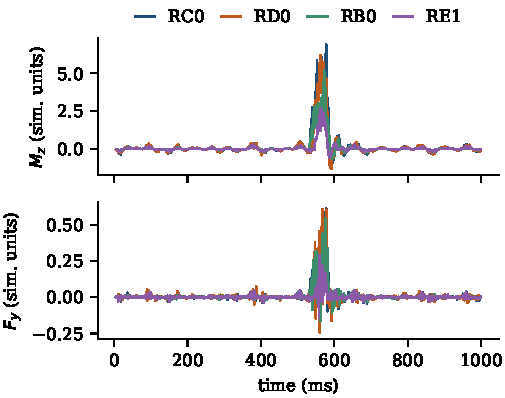
\includegraphics[width=\columnwidth]{figs/fig_signals.pdf}
\caption{Example of the signals for one simulation of dataset~P (peg at $x=14.0$, $y=12.7$~mm): bending moment $M_z$ and transverse force $F_y$ at the base of the four whiskers with the strongest contact over 1~s of whisking (eight whisk cycles).}
\label{fig:signals}
\end{figure}

\subsection{Datasets}
Table~\ref{tab:datasets} summarizes the four datasets.

\textbf{Dataset P (peg localization).} A static vertical peg is placed at a position sampled uniformly in $x\in[12,42]$~mm, $y\in[9,31]$~mm, excluding two corners that the array cannot reach. The label is the peg position $(x,y)$.

\textbf{Datasets D1--D3 (shape and position).} The object is one of nine meshes from three families (cylinder, rectangular prism, wall with a sinusoidal front), three sizes each, placed with a random position and yaw. The labels are the shape family and the position. Before simulating, every candidate pose is checked geometrically using the footprint of the whiskers at rest and over one whisk cycle: a pose is rejected if the object intersects a resting whisker, which would start the simulation in penetration, or if the whisking sweep never reaches the object.

The three datasets differ in how poses are assigned:
\begin{itemize}
\item \textbf{D1 (static head, pose-coupled).} A mesh and a pose are sampled together and the pair is accepted if valid. Sizes differ strongly between families (cylinder radii 1--5~mm, prisms up to $6\times20$~mm, walls up to 25~mm long).
\item \textbf{D2 (static head, pose-decoupled).} The pose is sampled first and accepted only if it is valid for all nine meshes; the mesh is then assigned at random in a balanced way. The families are given comparable sizes (cylinder radii 4--6~mm; prisms $8\times8$, $6\times12$ and $10\times10$~mm; walls 12~mm long with amplitudes 1.5--2.5~mm) and all objects are 160~mm tall so that every whisker row can reach them.
\item \textbf{D3 (approaching head, pose-decoupled).} As D2, but the head advances towards the object at 60~mm/s, about 28~mm during the simulation, so that whiskers are pushed against the object instead of grazing it with their tips. Poses must in addition keep the object ahead of the head at all times.
\end{itemize}

\begin{table}[t]
\caption{Datasets generated for this study}
\label{tab:datasets}
\centering
\setlength{\tabcolsep}{4pt}
\begin{tabular}{@{}lcccc@{}}
\toprule
 & P & D1 & D2 & D3 \\
\midrule
Object & peg & 9 meshes & 9 meshes & 9 meshes \\
Head & static & static & static & approaching \\
Shape indep. of pose & -- & no & yes & yes \\
Simulations & 300 & 300 & 306 & 306 \\
Duration (s) & 1.0 & 1.0 & 0.5 & 0.5 \\
With contact & 283 & 284 & 272 & 275 \\
Median peak moment & 4.5 & 2.2 & 1.5 & 2.7 \\
\bottomrule
\end{tabular}
\end{table}

\subsection{Models}
\textbf{CNN--LSTM.} Two one-dimensional convolutions over time (64 filters, kernel 5, batch normalization, ReLU) followed by max pooling, a bidirectional LSTM with 64 units per direction, temporal average pooling and a two-layer head. It has 148k parameters. The 162 input channels are the 27 whiskers times six signals.

\textbf{TCN.} Five convolutional levels with kernel 5 and dilations 1, 2, 4, 8 and 16 (64 filters, batch normalization, ReLU, dropout 0.2), followed by temporal average pooling and the same head (139k parameters). Because complete simulations are analysed offline, the convolutions are not causal.

\textbf{Non-temporal baselines.} (i) The training mean or majority class. (ii) Ridge regression on the mean, standard deviation and maximum absolute value of each channel. (iii) A random forest~\cite{breiman2001} with 400 trees on the \emph{contact map}, the maximum absolute moment of each whisker over the simulation, which discards all temporal structure.

\textbf{Pose-only control.} For shape classification we also train a random forest that receives only the true object pose $(x,y,\text{yaw})$ and never sees the mechanical signals. It is not a competitor: its accuracy measures how much of the shape label can be guessed from where the object is, that is, the size of any shortcut introduced by the data design.

For shape and position the networks have two heads, three logits for the shape family and two outputs for position, trained with cross-entropy plus ten times the mean squared error. Yaw is not predicted because it is not uniquely defined for cylinders and symmetric prisms.

\subsection{Evaluation protocol}
The unit of partition is the simulation. We use five-fold cross-validation (stratified by class for D1--D3); within each training fold, 20\% of the simulations are held out for early stopping, and the test fold is evaluated once. Each channel is standardized with the mean and standard deviation of the training simulations only. Networks are trained with Adam~\cite{kingma2015} (learning rate $10^{-3}$, weight decay $10^{-4}$, batch size 8), learning-rate reduction on plateau and early stopping, and each fold is repeated with several random seeds (three for dataset~P, two elsewhere). Position labels are divided by 50~mm for training. Unless stated otherwise, signals are subsampled to 500~Hz. We report the mean Euclidean position error in millimetres and the classification accuracy, as mean~$\pm$~standard deviation over folds and seeds.

Robustness is measured by evaluating models trained on clean data on perturbed test simulations: additive Gaussian noise with standard deviation equal to 5, 10 or 20\% of the training standard deviation of each channel, amplitude scaling by 0.8 or 1.2, and temporal shifts of $\pm5$ samples.

\section{Results}
\subsection{Peg localization}
Table~\ref{tab:peg} gives the position error on the 283 simulations of dataset~P with contact. At 500~Hz the CNN--LSTM reaches \pmsd{1.76}{0.14}~mm and the random forest on the contact map \pmsd{1.71}{0.28}~mm, against 9.47~mm for the training mean and 3.77~mm for ridge regression. The two best models are statistically indistinguishable; the network has a lower spread across folds. For the CNN--LSTM the coefficient of determination is 0.95 for $x$ and 0.94 for $y$. Fig.~\ref{fig:scatter} shows the predictions over the workspace: the median error is 1.16~mm and the largest errors occur at the edge of the reachable region. The remaining 17 simulations had no contact and cannot be localized by any model; they mark the observability limit of the array.

\begin{table}[t]
\caption{Peg localization: position error (mm) by sampling rate}
\label{tab:peg}
\centering
\begin{tabular}{@{}lccc@{}}
\toprule
Model & 100 Hz & 200 Hz & 500 Hz \\
\midrule
Training mean & \pmsd{9.47}{0.45} & \pmsd{9.47}{0.45} & \pmsd{9.47}{0.45} \\
Ridge on channel statistics & \pmsd{3.84}{0.58} & \pmsd{3.85}{0.39} & \pmsd{3.77}{0.72} \\
RF on contact map & \pmsd{1.97}{0.28} & \pmsd{1.87}{0.33} & \pmsd{1.71}{0.28} \\
CNN--LSTM & \pmsd{2.15}{0.18} & \pmsd{2.08}{0.22} & \pmsd{1.76}{0.14} \\
\bottomrule
\end{tabular}
\end{table}

\begin{figure}[t]
\centering
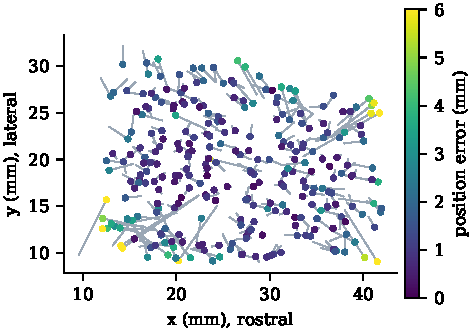
\includegraphics[width=\columnwidth]{figs/fig_scatter.pdf}
\caption{Peg localization with the CNN--LSTM at 500~Hz (test predictions of all folds, one seed). Each dot is the true peg position, coloured by error; the line joins it to the predicted position.}
\label{fig:scatter}
\end{figure}

\textbf{Architecture and loss.} Table~\ref{tab:ablation} compares variants under a common protocol. All compact models lie between 1.4 and 1.9~mm and their differences are of the order of the variation across folds. The TCN is the most accurate (\pmsd{1.44}{0.32}~mm) and mean squared error is a better loss than the smooth L1 loss at this label scale. A loss that adds a one-dimensional structural similarity term~\cite{wang2004} to the mean squared error is unstable for a two-dimensional output: two of ten runs diverged. Model size did not translate into accuracy: a variant with three stacked bidirectional LSTM layers of 512, 256 and 128 units (6.4M parameters), evaluated on a single fold at 200~Hz because of its cost, reached 3.48~mm, against about 2.0~mm for the compact CNN--LSTM on the same fold, with roughly 120 times the training time.

\begin{table}[t]
\caption{Peg localization: architecture and loss variants (500 Hz, five folds, two seeds)}
\label{tab:ablation}
\centering
\begin{tabular}{@{}llcc@{}}
\toprule
Model & Loss & Error (mm) & Parameters \\
\midrule
TCN & smooth L1 & \pmsd{1.44}{0.32} & 139k \\
CNN--LSTM & MSE & \pmsd{1.54}{0.16} & 148k \\
BiLSTM only & smooth L1 & \pmsd{1.76}{0.27} & 125k \\
CNN--LSTM & smooth L1 & \pmsd{1.81}{0.19} & 148k \\
CNN only & smooth L1 & \pmsd{1.84}{0.16} & 77k \\
CNN--LSTM & MSE + SSIM & median 1.95$^{\ast}$ & 148k \\
\bottomrule
\multicolumn{4}{@{}l}{\footnotesize $^{\ast}$Two of ten runs diverged (errors of 10 and 38 mm).}
\end{tabular}
\end{table}

\textbf{Robustness.} Table~\ref{tab:robust} and Fig.~\ref{fig:noise} show the main difference between the temporal model and the static summary. The error of the CNN--LSTM is unchanged by additive noise up to 20\% of the channel standard deviation (1.84~mm), whereas the random forest on the contact map degrades to 5.65~mm, a factor of 3.3. The contact map is built from maxima, which noise biases upwards, while the network integrates the whole sequence. Amplitude scaling affects both models similarly, and neither is sensitive to a shift of $\pm5$ samples; the contact map is invariant to shifts by construction.

\begin{table}[t]
\caption{Peg localization: position error (mm) under test-time perturbations (500 Hz, five folds)}
\label{tab:robust}
\centering
\begin{tabular}{@{}lcc@{}}
\toprule
Condition & CNN--LSTM & RF on contact map \\
\midrule
Clean & \pmsd{1.84}{0.20} & \pmsd{1.71}{0.28} \\
Noise 5\% & \pmsd{1.84}{0.19} & \pmsd{2.41}{0.34} \\
Noise 10\% & \pmsd{1.84}{0.19} & \pmsd{3.75}{0.47} \\
Noise 20\% & \pmsd{1.84}{0.17} & \pmsd{5.65}{0.61} \\
Amplitude $\times0.8$ & \pmsd{2.34}{0.25} & \pmsd{2.21}{0.25} \\
Amplitude $\times1.2$ & \pmsd{2.04}{0.18} & \pmsd{2.62}{0.16} \\
Shift $+5$ samples & \pmsd{1.86}{0.19} & \pmsd{1.71}{0.28} \\
Shift $-5$ samples & \pmsd{1.90}{0.21} & \pmsd{1.71}{0.28} \\
\bottomrule
\end{tabular}
\end{table}

\begin{figure}[t]
\centering
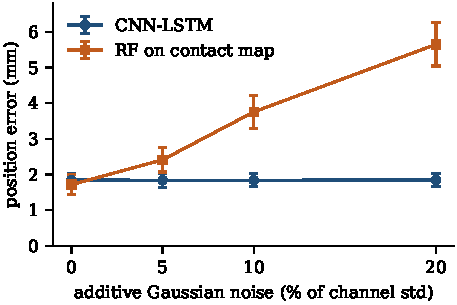
\includegraphics[width=\columnwidth]{figs/fig_noise.pdf}
\caption{Position error on dataset~P as a function of additive test noise. Error bars are the standard deviation over folds.}
\label{fig:noise}
\end{figure}

\subsection{Shape and position of objects}
\label{sec:shape}
Table~\ref{tab:shape} and Fig.~\ref{fig:shape} report the results on D1--D3.

\textbf{A design shortcut (D1).} On D1 the models appear to recognise shape: the random forest reaches an accuracy of 0.70 and the CNN--LSTM 0.68. The pose-only control, which never sees the signals, reaches 0.62. The geometric validity check had tied shape to position, because larger objects only fit farther from the head: the mean $x$ was 39.7~mm for cylinders, 40.6~mm for prisms and 43.5~mm for walls. The models with torque add only 3 to 8 points over that control, and most of what looks like shape recognition is recognition of where the object is.

\textbf{Decoupled design, static head (D2).} When poses are valid for every mesh and the mesh is assigned afterwards, the pose-only control falls to chance (\pmsd{0.36}{0.07}; 0.29 when computed on the pose list before simulating). No model then separates from chance: 0.39 for both the random forest and the CNN--LSTM, and 0.37 for the TCN, with confusion matrices spread evenly over the three classes.

\textbf{Decoupled design, approaching head (D3).} Moving the head towards the object raises the median peak moment from 1.5 to 2.7 and the largest values from about 5 to 14, so contacts are no longer limited to the whisker tips. Shape accuracy does not change: 0.36 for the random forest and 0.38 for both networks, against 0.36 for the pose-only control. A random forest with richer per-channel descriptors (mean, standard deviation, extrema, time of the peak and largest increment) reaches \pmsd{0.39}{0.05}. Restricting the analysis to the 93 simulations with the strongest contact gives \pmsd{0.44}{0.10}, and the binary problem cylinder versus wall on strong-contact simulations gives \pmsd{0.61}{0.12} against a chance level of 0.50. These values suggest a weak dependence on contact strength but are within the variation across folds.

\textbf{Position.} In contrast, object position is recovered in all three datasets. The random forest on the contact map gives \pmsd{1.78}{0.11}~mm on D2 and \pmsd{2.56}{0.17}~mm on D3, where the range of positions is wider and the training-mean error is 11.15~mm. The networks are less accurate than the random forest on these datasets (3.1--5.9~mm), which have about 220 training simulations per fold and a weaker signal than dataset~P.

\begin{table}[t]
\caption{Shape accuracy (chance 0.333) and position error for objects of three shape families}
\label{tab:shape}
\centering
\setlength{\tabcolsep}{4pt}
\begin{tabular}{@{}lccc@{}}
\toprule
 & D1 & D2 & D3 \\
\midrule
\multicolumn{4}{@{}l}{\emph{Shape accuracy}} \\
Majority class & 0.35 & 0.35 & 0.34 \\
Pose-only control & \pmsd{0.62}{0.05} & \pmsd{0.36}{0.07} & \pmsd{0.36}{0.06} \\
RF on contact map & \pmsd{0.70}{0.03} & \pmsd{0.39}{0.08} & \pmsd{0.36}{0.04} \\
CNN--LSTM & \pmsd{0.68}{0.08} & \pmsd{0.39}{0.05} & \pmsd{0.38}{0.04} \\
TCN & \pmsd{0.65}{0.08} & \pmsd{0.37}{0.04} & \pmsd{0.38}{0.05} \\
\midrule
\multicolumn{4}{@{}l}{\emph{Position error (mm)}} \\
Training mean & \pmsd{4.94}{0.29} & \pmsd{7.07}{0.79} & \pmsd{11.15}{0.79} \\
RF on contact map & \pmsd{3.30}{0.27} & \pmsd{1.78}{0.11} & \pmsd{2.56}{0.17} \\
CNN--LSTM & \pmsd{4.11}{0.30} & \pmsd{3.15}{0.60} & \pmsd{5.11}{0.57} \\
TCN & \pmsd{5.31}{1.08} & \pmsd{3.90}{0.70} & \pmsd{5.88}{0.73} \\
\bottomrule
\end{tabular}
\end{table}

\begin{figure}[t]
\centering
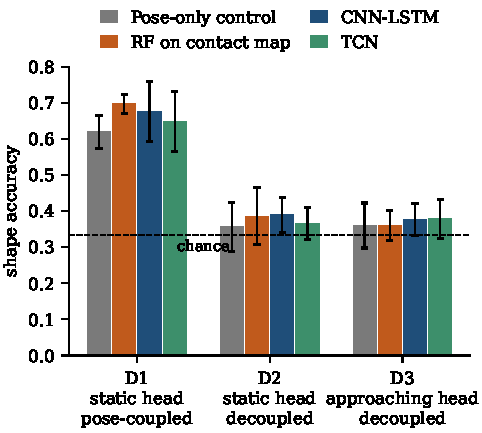
\includegraphics[width=\columnwidth]{figs/fig_shape.pdf}
\caption{Shape accuracy on the three designs. In D1 the pose-only control, which does not see the mechanical signals, already reaches 0.62. Once shape is independent of pose (D2, D3) all models are at chance, with a static or an approaching head.}
\label{fig:shape}
\end{figure}

\section{Discussion}
\textbf{Where versus what.} The base signals of the array carry robust information about object position. A static summary, the largest moment seen by each whisker, is enough to locate a peg within 2~mm, which agrees with the classical picture in which the pattern of which whiskers touch and how strongly encodes location~\cite{kaneko1998,birdwell2007}. Shape is a different matter. The three families used here differ by a few millimetres at the scale of a single object, while neighbouring whiskers are separated by several millimetres and each contact lasts a fraction of a whisk cycle. With the head static the objects must lie beyond the reach of the resting array to avoid initial penetration, so only whisker tips touch them; with the head approaching, contact is stronger but still consists of a short sequence of touches at an unknown orientation. In both regimes the signals of the three families are not separable by any of the models tested, including one that only summarises contact and two that use the full dynamics. We therefore attribute the result to the information content of the signal in this contact regime and not to model capacity.

\textbf{When temporal models matter.} On clean data, modelling the dynamics did not improve localization over the contact map, and all compact architectures performed alike. The benefit of the temporal model appears under sensor noise, where it keeps its accuracy and the summary based on maxima does not. For a physical sensor this is the more relevant comparison.

\textbf{Pose-only controls.} The shortcut in D1 arose from a reasonable step, rejecting invalid poses per object, and would have gone unnoticed in a standard evaluation, since accuracy was well above chance and the confusion matrix looked plausible. A classifier that sees only the nuisance variables costs seconds to train, can be run on the pose list before any simulation, and bounds how much of a result may be a shortcut~\cite{geirhos2020}. We suggest reporting it whenever labels and object placement are generated jointly.

\textbf{Limitations.} All results come from simulation with one whisking trajectory, one side of the face and the average rat morphology. Datasets have about 300 simulations each, which is small for sequence models and may explain why networks trail the random forest on D2 and D3. The shape families and sizes are specific; larger or more distinct objects may be separable. Noise robustness was measured for the CNN--LSTM and the random forest, not for the TCN, and the large stacked-LSTM variant was evaluated on a single fold. Signals are in simulator units and no sensor model is applied.

\section{Conclusion}
From newly generated simulations of an actively whisking 27-whisker array, the moments and forces at the whisker base allow the position of a peg to be recovered with an error of 1.4 to 1.8~mm, and the position of small objects with 1.8 to 2.6~mm. A CNN--LSTM is as accurate as a static contact map on clean data and markedly more robust to noise. The shape family of small objects could not be discriminated once shape and pose were decoupled, under two contact regimes, and a pose-only control was needed to detect that an earlier design had produced a spurious accuracy of 0.70. Future work should test contact regimes that trace the object surface, such as lateral sweeps of the head, larger datasets, objects with larger geometric differences and representations that exploit the spatial arrangement of the whiskers.

\section*{Data and Code Availability}
The simulator patches, dataset generators, training scripts, notebooks and result files are available at \url{https://github.com/clondonoidarraga/whisker-torque-profile}.

\begin{thebibliography}{00}
\bibitem{mitchinson2011} B. Mitchinson \emph{et al.}, ``Active vibrissal sensing in rodents and marsupials,'' \emph{Philos. Trans. R. Soc. B}, vol. 366, no. 1581, pp. 3037--3048, 2011.
\bibitem{kaneko1998} M. Kaneko, N. Kanayama, and T. Tsuji, ``Active antenna for contact sensing,'' \emph{IEEE Trans. Robot. Autom.}, vol. 14, no. 2, pp. 278--291, 1998.
\bibitem{solomon2006} J. H. Solomon and M. J. Hartmann, ``Robotic whiskers used to sense features,'' \emph{Nature}, vol. 443, no. 7111, p. 525, 2006.
\bibitem{pearson2011} M. J. Pearson, B. Mitchinson, J. C. Sullivan, A. G. Pipe, and T. J. Prescott, ``Biomimetic vibrissal sensing for robots,'' \emph{Philos. Trans. R. Soc. B}, vol. 366, no. 1581, pp. 3085--3096, 2011.
\bibitem{lepora2018} N. F. Lepora, M. J. Pearson, and L. Cramphorn, ``TacWhiskers: Biomimetic optical tactile whiskered robots,'' in \emph{Proc. IEEE/RSJ Int. Conf. Intell. Robots Syst. (IROS)}, 2018, pp. 7628--7634.
\bibitem{birdwell2007} J. A. Birdwell \emph{et al.}, ``Biomechanical models for radial distance determination by the rat vibrissal system,'' \emph{J. Neurophysiol.}, vol. 98, no. 4, pp. 2439--2455, 2007.
\bibitem{huet2017} L. A. Huet, J. W. Rudnicki, and M. J. Z. Hartmann, ``Tactile sensing with whiskers of various shapes: Determining the three-dimensional location of object contact based on mechanical signals at the whisker base,'' \emph{Soft Robot.}, vol. 4, no. 2, pp. 88--102, 2017.
\bibitem{zweifel2021} N. O. Zweifel, N. E. Bush, I. Abraham, T. D. Murphey, and M. J. Z. Hartmann, ``A dynamical model for generating synthetic data to quantify active tactile sensing behavior in the rat,'' \emph{Proc. Natl. Acad. Sci. U.S.A.}, vol. 118, no. 27, e2011905118, 2021.
\bibitem{coumans2015} E. Coumans, ``Bullet physics simulation,'' in \emph{ACM SIGGRAPH 2015 Courses}, 2015.
\bibitem{hochreiter1997} S. Hochreiter and J. Schmidhuber, ``Long short-term memory,'' \emph{Neural Comput.}, vol. 9, no. 8, pp. 1735--1780, 1997.
\bibitem{bai2018} S. Bai, J. Z. Kolter, and V. Koltun, ``An empirical evaluation of generic convolutional and recurrent networks for sequence modeling,'' arXiv:1803.01271, 2018.
\bibitem{kapoor2023} S. Kapoor and A. Narayanan, ``Leakage and the reproducibility crisis in machine-learning-based science,'' \emph{Patterns}, vol. 4, no. 9, 100804, 2023.
\bibitem{geirhos2020} R. Geirhos \emph{et al.}, ``Shortcut learning in deep neural networks,'' \emph{Nat. Mach. Intell.}, vol. 2, no. 11, pp. 665--673, 2020.
\bibitem{breiman2001} L. Breiman, ``Random forests,'' \emph{Mach. Learn.}, vol. 45, no. 1, pp. 5--32, 2001.
\bibitem{kingma2015} D. P. Kingma and J. Ba, ``Adam: A method for stochastic optimization,'' in \emph{Proc. Int. Conf. Learn. Represent. (ICLR)}, 2015.
\bibitem{wang2004} Z. Wang, A. C. Bovik, H. R. Sheikh, and E. P. Simoncelli, ``Image quality assessment: From error visibility to structural similarity,'' \emph{IEEE Trans. Image Process.}, vol. 13, no. 4, pp. 600--612, 2004.
\end{thebibliography}

\end{document}
